% File: intro.tex
% Date: Mon Dec 30 14:18:15 2013 +0800
% Author: Yuxin Wu <ppwwyyxxc@gmail.com>
\section{Introduction}
This is an image retargeting program using Seam Carving\cite{sc} algorithm.

\subsection{Compilation}
Dependencies:

\begin{enumerate}
    \item gcc >= 4.7
    \item GNU make
    \item Magick++
\end{enumerate}

Compilation:
\begin{lstlisting}
$ make
\end{lstlisting}

\subsection{Run}
The program supports following command line arguments:
\begin{lstlisting}
  -i <file>   input image file
  -o <file>   output image file
  -w <num>   target width. can be the pixel number in integer, or a relative number in (0, 1]
  -h <num>   target height. same as above
  -e <file>   energy file, optional
  -m <file>   mask image, red to discard, green to keep. optional
  -c <type>   convolution type, can be one of 'prewitt', 'vsquare', 'sobel', 'laplacian'
  -p    use optimized seam carving.
  -f <file>   feature file. every line is a coordinate.
  -v    output intermidiate results to generate video demo.
\end{lstlisting}

\subsection{Examples}
\begin{enumerate}

  \item Output with every intermidiate result:

    \begin{lstlisting}
$ ./image_resize -i ./sea.png -o result.png -w 0.8 -v
$ feh path*.png
    \end{lstlisting}

    The original image and the result is as followed:

    \begin{figure}[H]
        \centering
        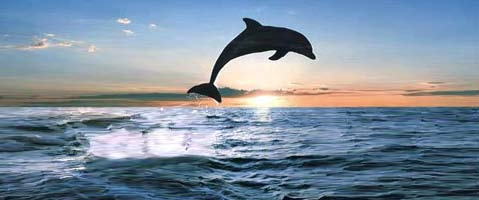
\includegraphics[width=0.9\textwidth]{src/sea.png}
    \end{figure}
    \begin{figure}[H]
        \centering
        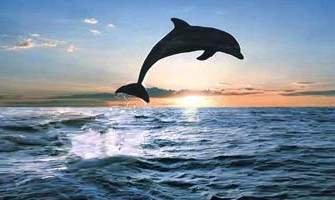
\includegraphics[width=0.63\textwidth]{result/sea.png}
    \end{figure}

  \item Use mask:
    \begin{lstlisting}
$ ./image_resize -i mike.jpg -o result.png -w 0.8 -m mike-m.png
    \end{lstlisting}
\end{enumerate}
